\chapter{Anhang}

\section{MRiLab auf "GPU-Rechner"}%%%%%%%%%%%%%%%%%%%%%%%%%%%%%%%%%%
\label{sec:usedPC}
MRiLab wird auf einem Personal Computer mit der, in \autoref{tab:gpuPc} angegebenen, Hardware- und Software-Ausstattung installiert.

\begin{table}[H]
	\centering
	\caption{Spezifikationen des verwendeten Rechners}
	\begin{tabular}{ll}
		\toprule
		\multicolumn{2}{c}{\textbf{Hardware}} \\
		CPU & Intel Xeon E5-1650v4 (3.6 GHz) \\
		GPU & Nvidia GeForce GTX Titan X \\
		RAM & 2x8 GB \\
		\midrule
		\multicolumn{2}{c}{\textbf{Software}} \\
		OS & Microsoft Windows 10 Pro for Workstations \\
		MATLAB & R2018a \\
		GPU Driver & Nvidia 398.82 \\
		CUDA & 7.0 \\
		\bottomrule
	\end{tabular}
	\label{tab:gpuPc}
\end{table}

Andere getestete Konfigurationen:
\begin{enumerate}
	\item \textbf{Ubuntu 18.04, CUDA 9.2}: CUDA 9.2 unterstützt offiziell nur Ubuntu 16.04 und 17.10. Die Installation von CUDA war dennoch erfolgreich\footnote{siehe https://devtalk\-.nvidia.com/\-default/topic/983777/\-cuda-setup-and-installation\-/can-t-locate-installutils\--pm-in-inc/}. 
	Die CUDA Libraries werden aber von \texttt{DoScanAtGPU} in MRiLab nicht gefunden (Von MRiLab wird versucht libcudart.so.7 statt allgemein libcudart.so zu laden).
	
	\item\label{en:versuch2} \textbf{Ubuntu 18.04, CUDA 7.0}: CUDA 7.0 unterstützt offiziell nur Ubuntu 14.04, 14.10 und 12.04. Die Installation ist dennoch ohne Probleme möglich. Die CUDA Libraries werden von MRiLab gefunden und ein Scan kann gestartet werden. Gegen Ende der Simulation stürzt MATLAB jedoch aufgrund eines Laufzeitfehlers in \texttt{DoScanAtGPU} ab.
	
	\item \textbf{Ubuntu 16.04, CUDA 7.0}: Fehlerbild wie unter Punkt \ref{en:versuch2}.
	
	\item \textbf{Ubuntu 14.04, CUDA 7.0}: MATLAB bzw. MRiLAB aufgrund eines Bugs nicht benutzbar ("dlopen: cannot load any more object with static TLS")
	
\end{enumerate}

\clearpage
\section{Modifikationen MRiLab GUI}%%%%%%%%%%%%%%%%%%%%%%%%%%%%%%%%%
Für die, in dieser Arbeit vorgenommenen, Erweiterungen von MRiLab ist es von Vorteil, Simulationsparameter unkompliziert über die GUI anpassen zu können. Dazu müssen die gewünschten Bedienelemente in die bestehende GUI eingefügt werden.

\subsection{Struktur der MRiLab GUI}
MRiLab besteht aus einem Hauptfenster (\texttt{SimuPanel}) und mehreren Zusatzfenstern, den sog. "Design Panels". Das Haupt- und die Zusatzfenster sind jeweils mit dem MATLAB GUI Layout Editor \textit{GUIDE} (GUI development environment) erzeugt worden.

Ein GUIDE Fenster besteht aus zwei Dateien: Die .fig Binärdatei kann nur mit GUIDE geöffnet werden und enthält eine Beschreibung des Layouts. GUIDE erzeugt aus dieser eine MATLAB .m-Datei. Diese enthält Coderümpfe, um auf die im Layout spezifizierten Elemente zuzugreifen.

\subsubsection{Einbau eines neuen GUI-Elements}
Zum Einbau eines neuen GUI Elements in das MRiLab Hauptfenster wird GUIDE aus MATLAB heraus gestartet (\texttt{>>guide}) und die Datei \texttt{SimuPanel.fig} geöffnet. Nach dem Einfügen eines neuen Elements wird die Datei gespeichert. Die Datei \texttt{SimuPanel.m} wird dadurch im MATLAB Editor geöffnet und die "create"- bzw. "callback"-Funktion werden automatisch generiert.

\subsubsection{Zugriff auf neue GUI-Elemente}
GUIDE benutzt die Variable \texttt{handles}, um Daten zwischen GUI Elementen auszutauschen. Die Variable handles besteht aus einem Struct und kann auch für Benutzer-definierte globale Variablen benutzt werden. Dadurch ist der Zugriff aus allen GUI Teilen einfach möglich.

Auch, wenn die Programmierung mit globalen Variablen einige Probleme mit sich bringt\footnote{Programmteile schwierig isoliert zu testen, Auftreten von Namenskonflikten, etc.}, wird die oben erläuterte Vorgehensweise dennoch verwendet, um konsistent mit dem bestehenden Code zu sein.

Um aus einem Submodul (ohne GUI) auf ein Element des handles Struct zugreifen zu können, wird der Struct normal als Funktionsparameter übergeben.

\subsubsection{Beispiel}
Mit GUIDE wird ein Textfeld "phaseNoiseLevel" in das Hauptfenster eingebaut.
Auf den Wert in dem Textfeld soll aus \texttt{DoAddNoise.m} zugegriffen werden. \texttt{DoAddNoise.m} wird über \texttt{DoPostScan.m} von \texttt{SimuPanel.m} aufgerufen. Der handles Struct wird im Original MRiLab DoPostScan.m übergeben. Es muss daher lediglich der Parameterliste von \texttt{DoAddNoise.m} hinzugefügt werden.

\begin{listing}[H]
	\begin{minted}[fontsize=\footnotesize,linenos,autogobble]
	{Matlab}
	function DoAddNoise(handles)
	% Add noise in K-space data
	
	global VSig;
	global VCtl;
	
	uiPhaseNoiseLevel=str2num(get(handles.phaseNoiseLevel,'String'));
	...
	\end{minted}
	\caption{Beginn der Funktion \texttt{DoAddNoise.m} mit Zugriff auf \texttt{handles.phaseNoiseLevel}}
	\label{lst:doAddNoisesimuh}
\end{listing}

Ist die Definition von \texttt{DoAddNoise.m} um das "handles" Struct erweitert (siehe \autoref{lst:doAddNoisesimuh}), kann der Funktion das Struct von \texttt{DoPostScan.m} übergeben werden (\autoref{lst:doPostscansimuh}, Zeile 10).


\begin{listing}[H]
	\begin{minted}[fontsize=\footnotesize,linenos,autogobble]
	{Matlab}
	function DoPostScan(Simuh)
	
	global VCtl
	global VImg
	global VCoi
	DoUpdateInfo(Simuh,'Scan is complete!');
	set(Simuh.TimeWait_text,'String', ['Est. Time Left :  ' '~' ' : ' '~' ' : ' '~']);
	%% Signal Post-Processing
	%  Add noise
	DoAddNoise(Simuh);
	...
	\end{minted}
	\caption{Funktion \texttt{DoPostScan.m} übergibt "handles" Struct (mit Name "Simuh") an \texttt{DoAddNoise.m}}
	\label{lst:doPostscansimuh}
\end{listing}

\clearpage
\section{MRiLab Parameter}

\begin{table}[H]
	\caption{Für die Simulation relevante Parameter in MRiLab}
	\centering
	\begin{tabularx}{\textwidth}{l X l}
		\toprule
		\textbf{Name} & \textbf{Beschreibung} & \textbf{Einheit} \\
		\midrule
		FOVFreq & Größe des FOV in Richtung des Frequenzkodiergradienten & in \SI{}{\m}\\
		FOVPhase & Größe des FOV in Richtung des Phasenkodiergradienten & in \SI{}{\m}\\
		ResFreq & Auflösung in Richtung des Frequenzkodiergradienten & $\#Pixel/FOVFreq=\SI{}{\per\m}$\\
		ResPhase & Auflösung in Richtung des Phasenkodiergradienten & $\#Pixel/FOVPhase=\SI{}{\per\m}$\\
		SliceThick & Schichtdicke & \SI{}{\m}\\
		SliceNum & Anzahl der (symmetrisch um die gewählte Schicht) aufzunehmenden Schichten & - \\
		ScanPlane & Orientierung der $xy$-Ebene (Axial, Sagittal, Coronal) & - \\
		TR,TE & Repetitionszeit und Echozeit & \SI{}{\s}\\
		TEPerTR & Anzahl der aufzunehmenden Echos (aus verschiedenen Schichten, nur für Multiecho) & - \\
		Bandwidth & Bandbreite des Empfängers (entspricht dem inversen der Abtastrate $T_A$) & \SI{}{\hertz}\\
		NEX & Anzahl der aufeinander folgenden Aufnahmen zur Rauschunterdrückung durch Mittelung & - \\
		MaxSlewRate & Maximale Slewrate für alle Gradientenspulen & \SI{}{\tesla\per\m\per\s}\\
		MaxGrad & Maximale Stärke der Gradienten & \SI{}{\tesla\per\m}\\
		B0 & Feldstärke des statischen Magnetfeldes & \SI{}{\tesla}\\
		E1Level, B1Level & Stärke des RF-Feldes & (unbekannt)\\
		\bottomrule
	\end{tabularx}
	\label{tab:mriLabParam}
\end{table}

\clearpage
\section{MATLAB Funktion zum Erzeugen von Phasenrauschen im Zeitbereich}
\label{sec:addPhaseNoise}

\begin{longlisting}
	\begin{minted}[fontsize=\footnotesize,linenos,autogobble,breaklines]
	{Matlab}
	function [Sout,phi] = addPhaseNoise(Sin, fs, f_offset, P_dBc)
		[f_offset, k] = sort(f_offset);
		P_dBc = P_dBc(k);
		
		if(f_offset(1) ~= 0)
			f_offset = [0, f_offset]; 
			P_dBc = [ 0, P_dBc ];
		end
		
		N = length(Sin);
		if rem(N,2)
			M = (N+1)/2 + 1;
		else
			M = N/2 + 1;
		end
		
		freq  = linspace(0, fs/2, M);	
		df = fs/(2*M);
			
		% Perform interpolation of P_dBc in log-scale
		% source: https://de.mathworks.com/matlabcentral/
		% fileexchange/8844-phase-noise
		intrvlNum = length(f_offset);
		logP = zeros(1, M);
		for intrvlIndex = 1 : intrvlNum
			leftBound = f_offset(intrvlIndex);
			t1 = P_dBc(intrvlIndex);
			if intrvlIndex == intrvlNum
				rightBound = fs/2; 
				t2 = P_dBc(end);
				inside = find(freq>=leftBound & freq<=rightBound);  
			else
				rightBound = f_offset(intrvlIndex+1); 
				t2 = P_dBc(intrvlIndex+1);
				inside = find(freq>=leftBound & freq<rightBound);
			end	
			logP( inside ) = ...
			t1 + ( log10( freq(inside) + realmin) - log10(leftBound+ realmin) ) / ( log10( rightBound + realmin) - log10( leftBound + realmin)) * (t2-t1);     	
		end
		
		P = 10.^(real(logP)/10);	
		n = (sqrt(0.5)*(randn(1, M) +1j*randn(1, M)));	
		Phi = (2*M-2) * sqrt(df * P ) .* n; 	
		Phi M + (1:M-2)) = fliplr(conj(Phi(2:end-1))); 	
		Phi(1) = 0; 
		
		phi = real(ifft(Phi)); 	
		phase = exp(1j * phi(1:N));
			
		Sout = Sin .* phase;
	end
	\end{minted}
	\caption{Skript zur Kombination aller Einzelteile zu einem MRiLab Phantom}
	\label{lst:addPhaseNoise}
\end{longlisting}

\clearpage
\section{Kommerzielle MRT-Phantome}

\begin{table}[H]
	\caption[Kommerzielle MRT-Phantome]{Auswahl einiger am Markt verfügbarer MRT Phantome (Stand August 2018)}
	\centering
	\begin{tabularx}{\textwidth}{l X}
		\toprule
		\textbf{Abbildung} & \textbf{Beschreibung} \\
		\midrule \\[5pt]
		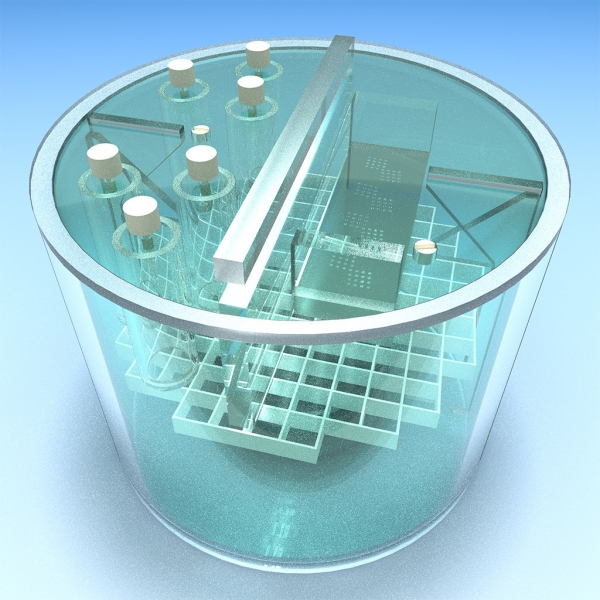
\includegraphics[width=0.25\textwidth,valign=t]{img/phantoms/allMRI.jpg} & \textbf{allMRI/\-Pro-MRI \newline180mm phantom} \newline Außendurchmesser: \SI{180}{\mm},\newline Höhe: \SI{150}{\mm} \newline \cite{allMRIphantom} \\
		&\\
		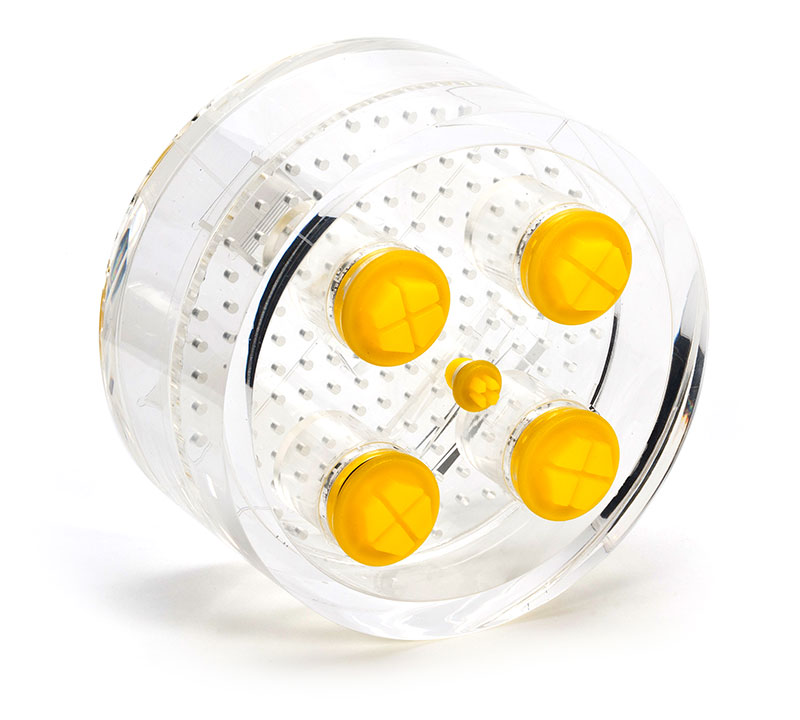
\includegraphics[width=0.25\textwidth,valign=t]{img/phantoms/MagIQ.jpg} & \textbf{Leeds MagIQ 142} \newline Außendurchmesser: \SI{142}{\mm},\newline Höhe: \SI{70}{\mm} \newline \cite{leeds} \\
		&\\
		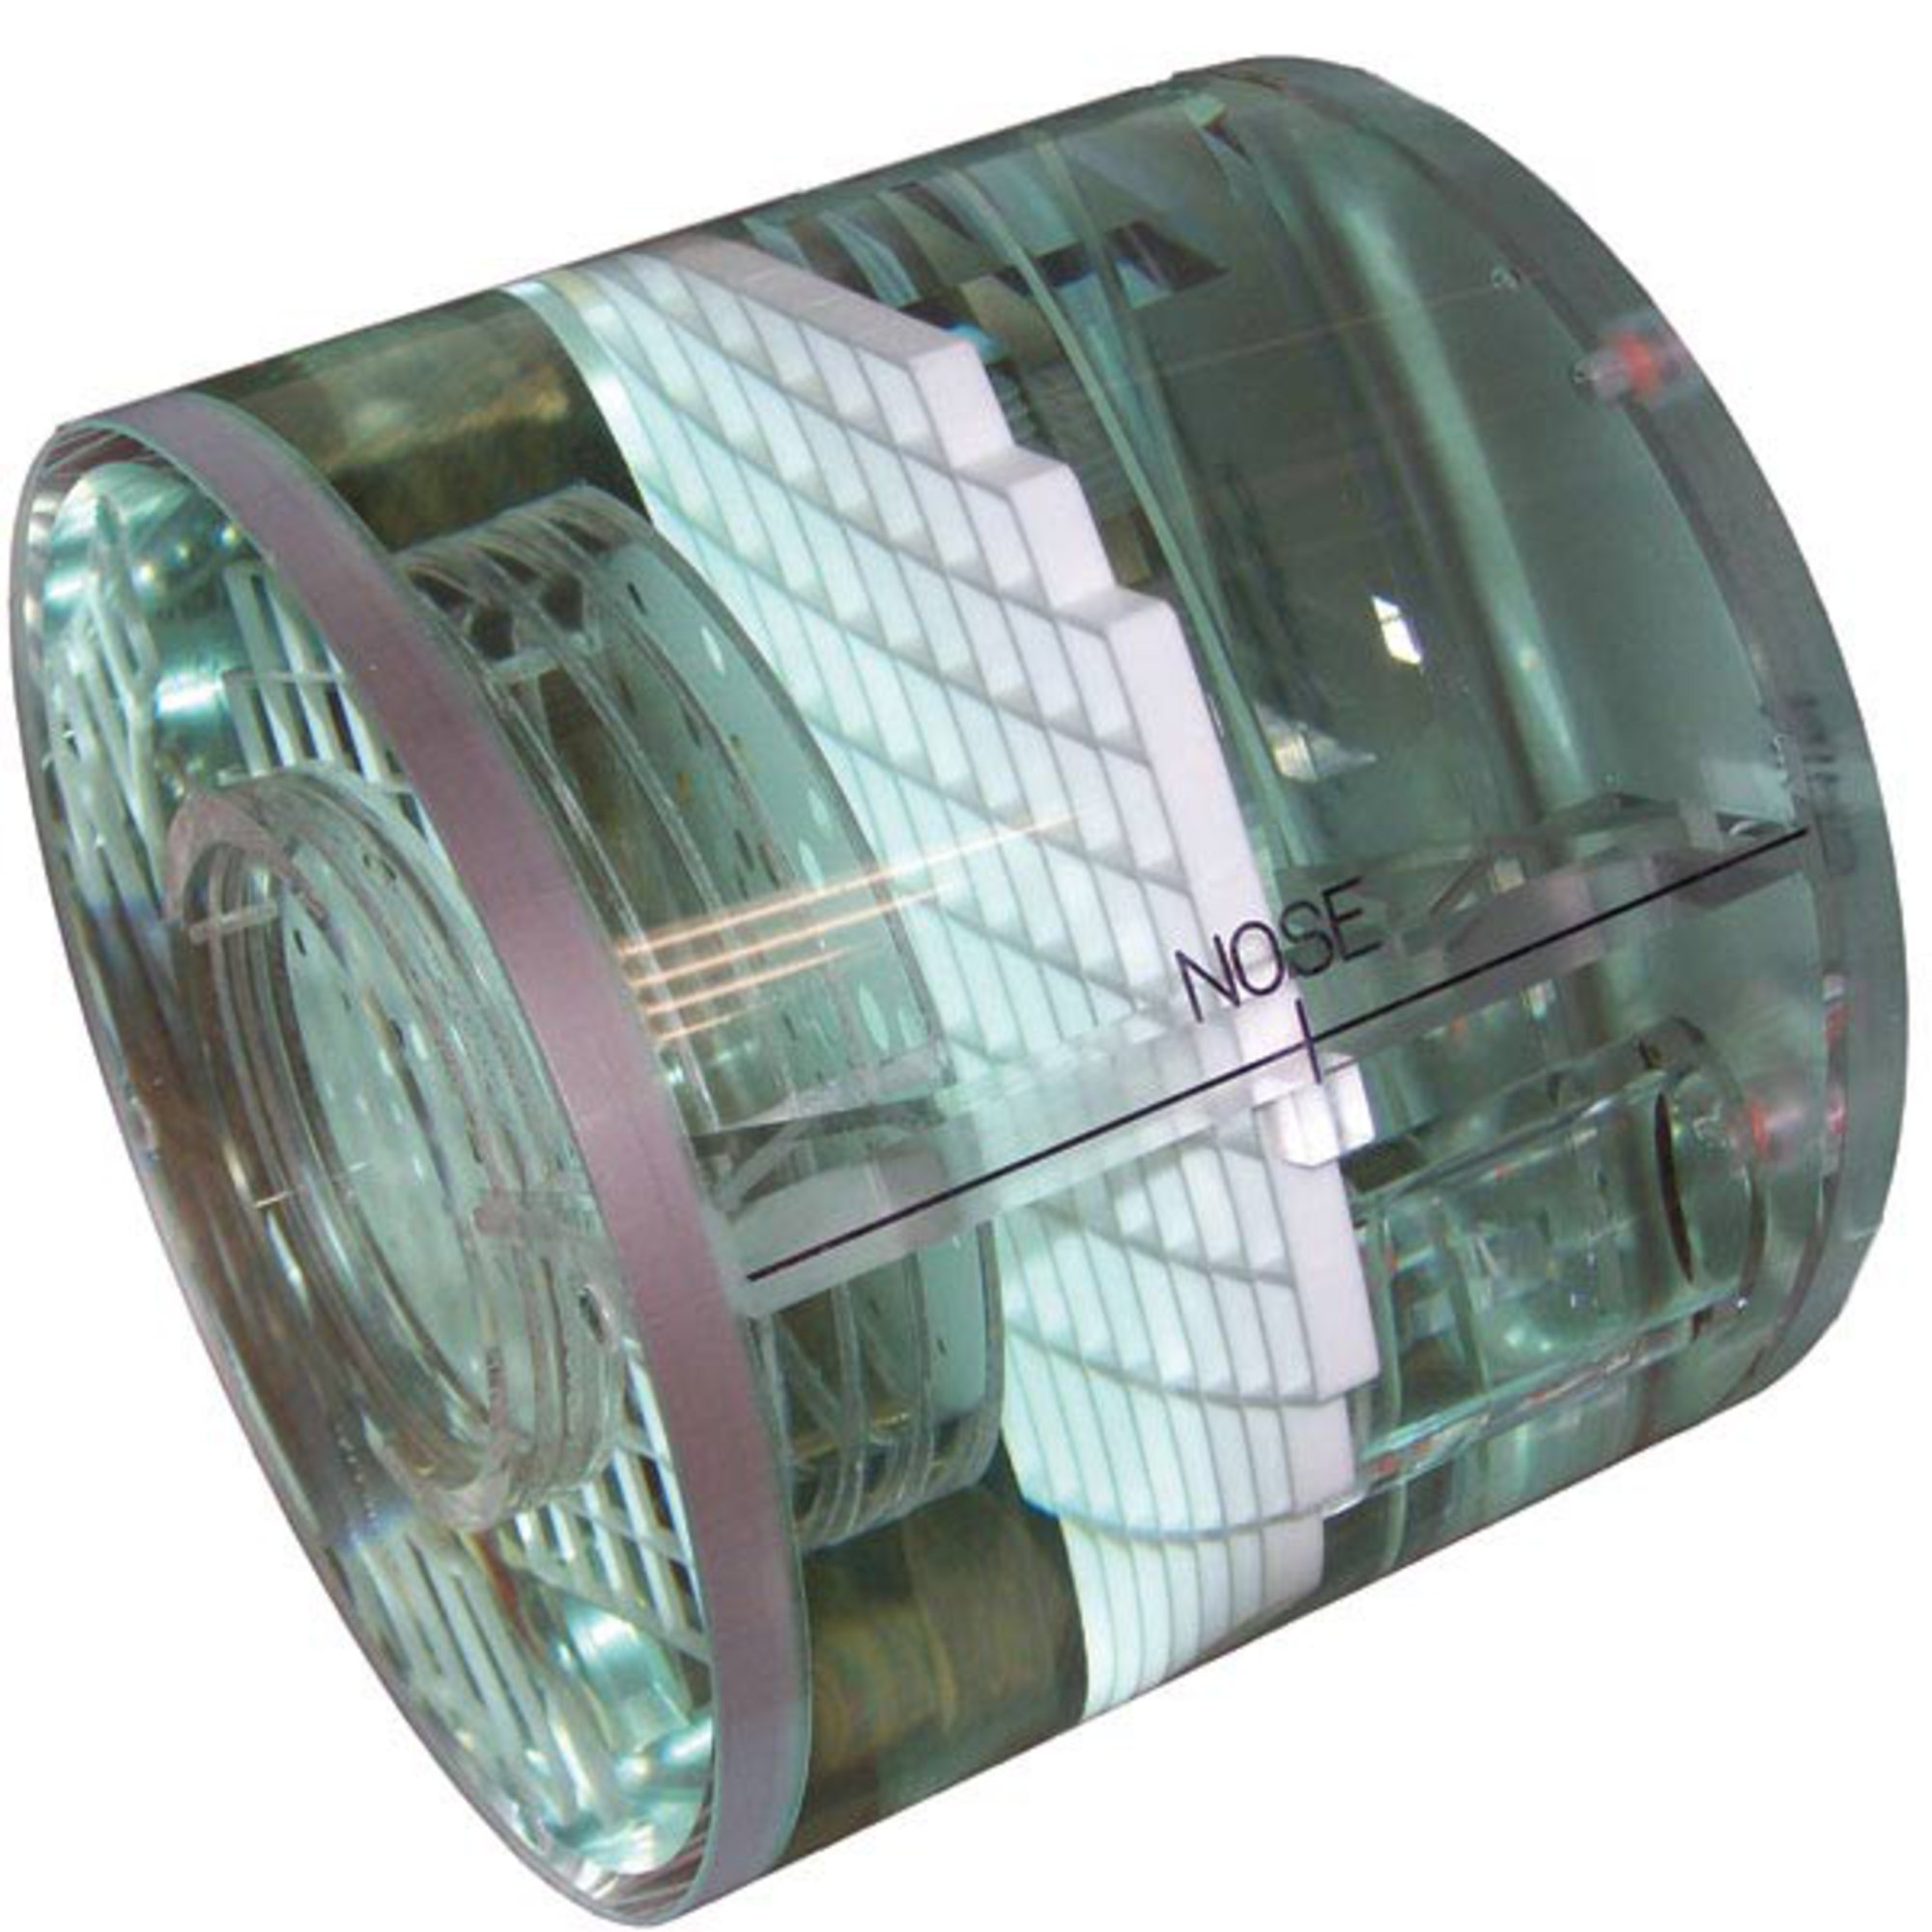
\includegraphics[width=0.25\textwidth,valign=t]{img/phantoms/acr.jpg} & \textbf{ACR MRI Phantom} \newline Außendurchmesser: \SI{203}{\mm},\newline Höhe: \SI{173.4}{\mm} \newline \cite{acr} \\
		&\\
		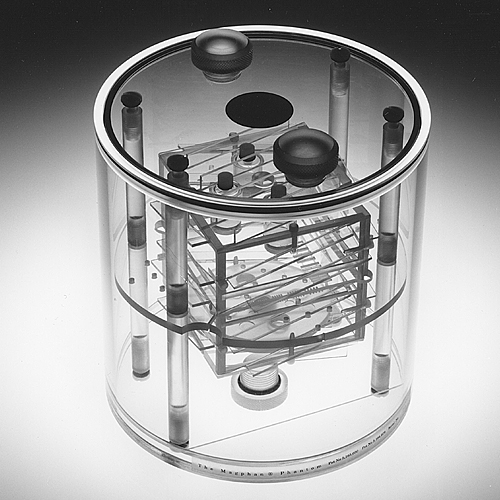
\includegraphics[width=0.25\textwidth,valign=t]{img/phantoms/Magphan.jpg} & \textbf{MAGPHAN CYLINDRICAL 170} \newline Außendurchmesser: \SI{200}{\mm} \newline \cite{mag170}  \\
		&\\
		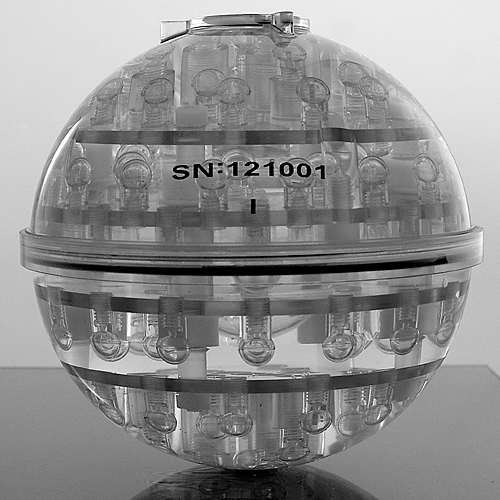
\includegraphics[width=0.25\textwidth,valign=t]{img/phantoms/magphan121.jpg} & \textbf{MAGPHAN MR Distortion Phantom (ADNI) 121} \newline Außendurchmesser: \SI{200}{\mm} \newline \cite{mag121} \\
		&\\
		\bottomrule
		\end{tabularx}
		\label{tab:phantomsOverview}
\end{table}

\clearpage		
\section{Fehlerbehebung in \texttt{stl-to-voxel}}
\label{sec:stlToVoxFix}
Untersuchungen zeigen, dass sich die Formatierung der von SolidWorks exportierten STL-Dateien (\autoref{lst:STLsw}) leicht von der im STL-Standard (\autoref{lst:STLspec}) unterscheidet: Zwischen den Koordinaten der Eckpunkten (Vertices) sind  zwei bzw. drei, statt ein Leerzeichen gesetzt. Dadurch scheitert der (Positions-basierte) Lesevorgang der Koordinaten in \texttt{stl\_reader.py}.

\begin{listing}[H]
	\begin{minted}[fontsize=\footnotesize,linenos,autogobble,showspaces]
	{C}
	solid cube_corner
	facet normal 0.0 -1.0 0.0
	outer loop
	vertex 0.0 0.0 0.0
	vertex 1.0 0.0 0.0
	vertex 0.0 0.0 1.0
	endloop
	endfacet
	...
	\end{minted}
	\caption{Auszug aus einer Standard-konformen STL-Datei}
	\label{lst:STLspec}
\end{listing}

\begin{listing}[H]
	\begin{minted}[fontsize=\footnotesize,linenos,autogobble,showspaces]
	{C}
	solid vcg
	facet normal  7.071068e-01  7.071068e-01  0.000000e+00
	outer loop
	vertex   1.351310e+01  1.431762e+02  1.100000e+02
	vertex   4.539159e+01  1.112977e+02  1.100000e+02
	vertex   1.351310e+01  1.431762e+02  1.050000e+02
	endloop
	endfacet
	...
	\end{minted}
	\caption{Auszug aus einer mit SolidWorks generierten STL-Datei}
	\label{lst:STLsw}
\end{listing}

Zur Fehlerbehebung wird ein Filter eingesetzt, der leere Zeichenketten ausfiltert (\autoref{lst:stlToVoxFix}).

\begin{listing}[H]
	\begin{minted}[fontsize=\footnotesize,linenos,autogobble,escapeinside=||]
	{Python}
	...
	words = line.strip().split(' ')
	|\colorbox{green!20}{words=list(filter(None,words))}| 
	assert words[0] == 'vertex'
	verticies.append((float(words[1]),
	float(words[2]),
	float(words[3])))
	...
	\end{minted}
	\caption{Modifikation der Datei \texttt{stl\_reader.py} zur Fehlerbehebung beim Lesen von "SolidWorks STL-Dateien"}
	\label{lst:stlToVoxFix}
\end{listing}

\clearpage
\section{MATLAB Skript zum Erzeugen einer MRiLab Phantomdatei}

\begin{longlisting}
	\begin{minted}[fontsize=\footnotesize,linenos,autogobble,breaklines]
	{Matlab}
	%this path contains subfolders with all materials in the phantom
	%each subfolder contains N png files and a property .txt file
	baseFolder='/home/ubuntu/matlabProjects/simulation/srcMyPhantom/out4';
	
	%desired file name for the phantom:
	phantomName='brukerBioSpinMRI63mm';
	
	%get all subfolders in the base path
	files = dir(baseFolder);
	dirFlags = [files.isdir];
	subFolders = files(dirFlags);
	subFolders(1:2)=[]; %remove '.' and '..' TODO: OS dependent?
	
	%get diemensions of first image in first sub folder and preallocate voxel matrices
	currFolder=fullfile(subFolders(1).folder,subFolders(1).name);
	pngFolderInfo=dir(fullfile(currFolder, '*.png'));
	pngPaths=fullfile({pngFolderInfo.folder},{pngFolderInfo.name});
	A=imread(cell2mat(pngPaths(1)));
	pngDimensions=size(A);
	Rho=zeros(pngDimensions(1),pngDimensions(2),length(pngPaths),'uint8');
	T1=zeros(pngDimensions(1),pngDimensions(2),length(pngPaths),'uint8');
	T2=zeros(pngDimensions(1),pngDimensions(2),length(pngPaths),'uint8');
	T2star=zeros(pngDimensions(1),pngDimensions(2),length(pngPaths),'uint8');
	
	%for loop over all sub folder containing all materials
	for k=1:length(subFolders) 
		currFolder=fullfile(subFolders(k).folder,subFolders(k).name);
		
		%get property scaling factors h_* for current material
		properties=importdata(fullfile(currFolder,'properties.txt'));
		keys=(properties.textdata);
		if(~(strcmp(keys{1},'Rho') && strcmp(keys{2},'T1') && strcmp(keys{3},'T2') && strcmp(keys{4},'T2*')))
			error('error in properties.txt')
		end
		h_Rho=properties.data(1);
		h_T1=properties.data(2);
		h_T2=properties.data(3);
		h_T2star=properties.data(4);
		
		%get png files in the current folder
		pngFolderInfo=dir(fullfile(currFolder, '*.png'));
		pngPaths=fullfile({pngFolderInfo.folder},{pngFolderInfo.name});
		if(isempty(pngPaths))
			error(['No .png files found in input folder "', pathToInputFolder,'"']); 
		end
		
		%loop over all the png images
		for l=1:length(pngPaths)
			disp([num2str(l),'/',num2str(length(pngPaths))]);
			Rho(:,:,l)=Rho(:,:,l)+h_Rho*(imread(cell2mat(pngPaths(l)))/255);
			T1(:,:,l)=T1(:,:,l)+h_T1*(imread(cell2mat(pngPaths(l)))/255);
			T2(:,:,l)=T2(:,:,l)+h_T2*(imread(cell2mat(pngPaths(l)))/255);
			T2star(:,:,l)=T2star(:,:,l)+h_T2star*(imread(cell2mat(pngPaths(l)))/255);
		end
	end
	
	%create MRiLab VObj
	
	stackSize=size(Rho);
	
	%MRIlab Phantom has to be a 1x1 struct named 'VObj' in file 'VObjSomething'
	VObj=struct;
	
	VObj.Gyro = 2.675380303797068e+08; %water
	VObj.ChemShift = 0; %assume no chemical shift
	
	VObj.XDim=stackSize(1);
	VObj.YDim=stackSize(2);
	VObj.ZDim=stackSize(3);
	
	VObj.XDimRes=0.001; %assume voxel sizes of 1mm
	VObj.YDimRes=0.001;
	VObj.ZDimRes=0.001;
	
	VObj.Type='Water';
	VObj.TypeNum=1;
	
	VObj.Rho=Rho;
	VObj.T1=T1;
	VObj.T2=T2;
	VObj.T2Star=T2star;
	
	%no data for Econ, MassDen available -> fill with Rho
	VObj.ECon(:,:,:,1)=Rho;
	VObj.ECon(:,:,:,2)=Rho;
	VObj.ECon(:,:,:,3)=Rho;
	VObj.MassDen=Rho;
	
	name=['VObj',phantomName];
	save(name,'VObj')
	
	disp(['phantom saved: ',name])
	\end{minted}
	\caption{Skript zur Kombination aller Einzelteile zu einem MRiLab Phantom}
	\label{lst:combinePhantomStacksIntoVoxelMatrix}
\end{longlisting}
